% Une ligne commentaire débute par le caractère « % »

\documentclass[a4paper]{article}

% Options possibles : 10pt, 11pt, 12pt (taille de la fonte)
%                     oneside, twoside (recto simple, recto-verso)
%                     draft, final (stade de développement)

\usepackage[utf8]{inputenc}   % LaTeX, comprends les accents !
\usepackage[T1]{fontenc}      % Police contenant les caractères français
\usepackage[francais]{babel}
\usepackage{fullpage}
\usepackage{multicol}
\usepackage{hyperref}
\hypersetup{
    colorlinks=true,
    linkcolor=blue,
    filecolor=magenta,      
    urlcolor=red
    }
% \urlstyle{same} % ça sert à rien ce truc
\usepackage{bookmark}
\usepackage{blindtext}



\usepackage{graphicx}  % pour inclure des images
\graphicspath{ {rapport/img/} }

%\pagestyle{headings}        % Pour mettre des entêtes avec les titres
                              % des sections en haut de page

\title{  TP2 : Les capteurs\\Programmation mobile}
\author{Mohamad Satea Almallouhi - Tony Nguyen\\\emph{M1 Génie Logiciel}\\Faculté des Sciences\\Université de Montpellier.}
\date{5 mars 2024}



\begin{document}
    \maketitle
    \begin{center}
    
\includegraphics[height=.95\textwidth]{makima_standing}
    \end{center}

    \begin{abstract}     % Résumé du travail
      \emph{Nous avons réalisé une application Android en Java afin de démontrer l'utilisation des capteurs intégré.}
    \end{abstract}
    \newpage
    %\dominitoc  % initializer les minitoc
    \tableofcontents

    \newpage
    \begin{multicols}{2}
        % [
        %     Faire une vidéo, le rapport avec des screenshot des résultats et du code et enfin un read.md(instruction). En plus, pour le bonus, faire une belle application, des tests unitaires, utiliser Kotlin, faire le rapport en Latex.
        % ]
        \section*{Introduction}
        \addcontentsline{toc}{section}{Introduction}
        \paragraph{}
            Dans ce TP, nous allons l'utilisation des capteurs intégré dans nos smartphones.
            
            Nous allons voir comment manipuler les différents types de capteur comme le GPS, la boussole, le gyroscope, etc ...
        \paragraph{}
            Pour réaliser ce tp, nous choisissons de créer une unique application avec un écran d'acceuil \emph{(ChoseApplication.java)} qui mène aux différentes activités correspondant à chaque exercice.
            
            \includegraphics[height=.8\textwidth]{screenshot}
        \paragraph{}
            Les sections du rapport suit les exercices.
        \section*{Démonstration}
        \addcontentsline{toc}{section}{Démonstration}
            \paragraph{}
            En ligne sur Youtube, à l'adresse URL \url{https://youtu.be/NjIdJrN-Rm8} une démonstration vidéo de notre travail.
        \section{Liste des capteurs \emph{(Index)}}
            \paragraph{}
                Lorsque l'on déploie une application sur un smarphone, nous ne pouvons pas être sûr des capteurs que l'on aura a notre disposition. Dans cette section, nous allons regarder tout les capteurs disponible sur un appareil donné.
            \paragraph{}
                Tout d'abord, il est nécessaire d'accèder au sensorManager par lequel les informations ainsi que l'accès aux capteurs passent.
                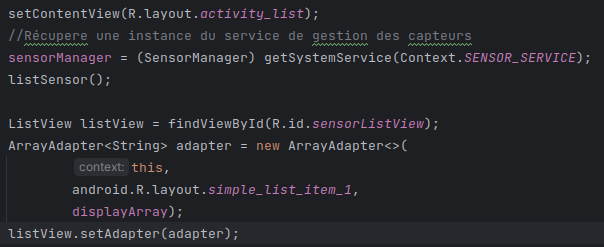
\includegraphics[width=.49\textwidth]{listeCapteur/sensorManager}
            \paragraph{}
                Ensuite, une fois qu'on a le sensorManager, nous pouvons faire appel à la fonction \textbf{getSensorList(Sensor.TYPE\_ALL)} qui nous renvoie un tableau de tous les capteurs.
                
                Pour accéder individuellement aux informations de chaque capteur représenté par un objet de type Sensor, nous invoquons les méthodes \textbf{getName(), getType() et getVersion()}.
                \noindent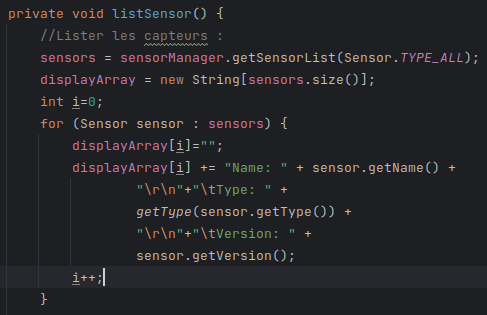
\includegraphics[width=.49\textwidth]{listeCapteur/listSensor}
            \paragraph{}
                Enfin, pour afficher à l'écran le résultat, nous utilisons une Vue de type ListView que nous avons au préalable déclarer dans le layout.
                \noindent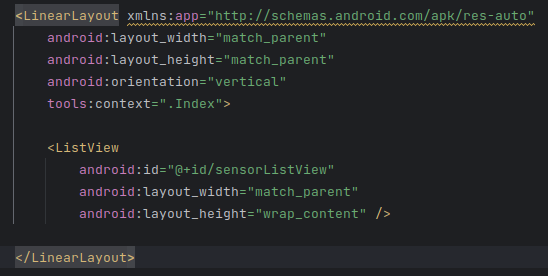
\includegraphics[width=.49\textwidth]{listeCapteur/layout}
                \noindent\includegraphics[width=.49\textwidth]{listeCapteur/screenshotSmall}
        \section{Détection de la disponibilité des capteurs \emph{(SensorAvailibility)}}
            \noindent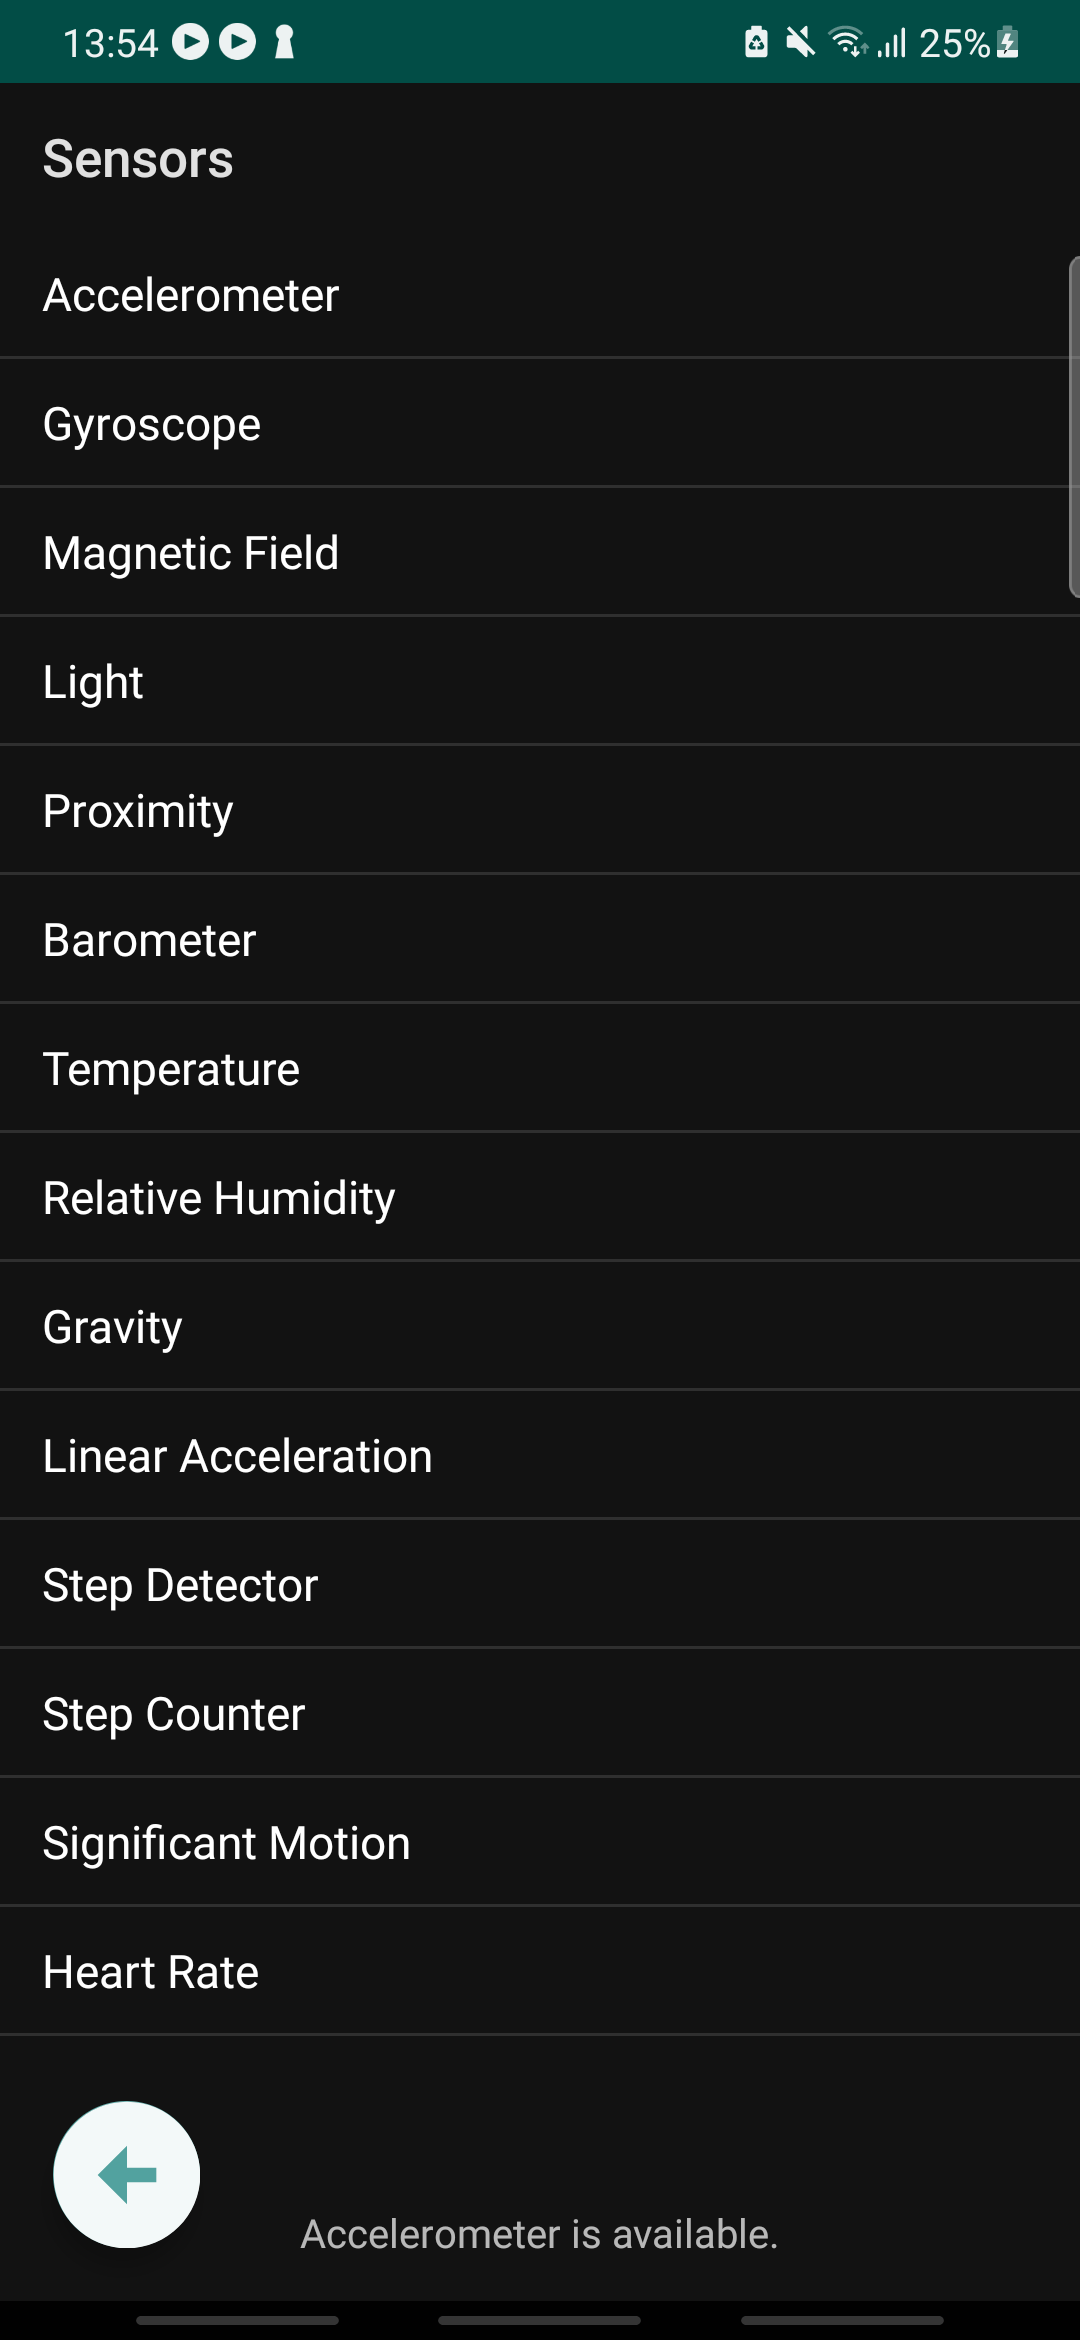
\includegraphics[height=.52\textwidth]{dispo/screenshotAvailable}
            \noindent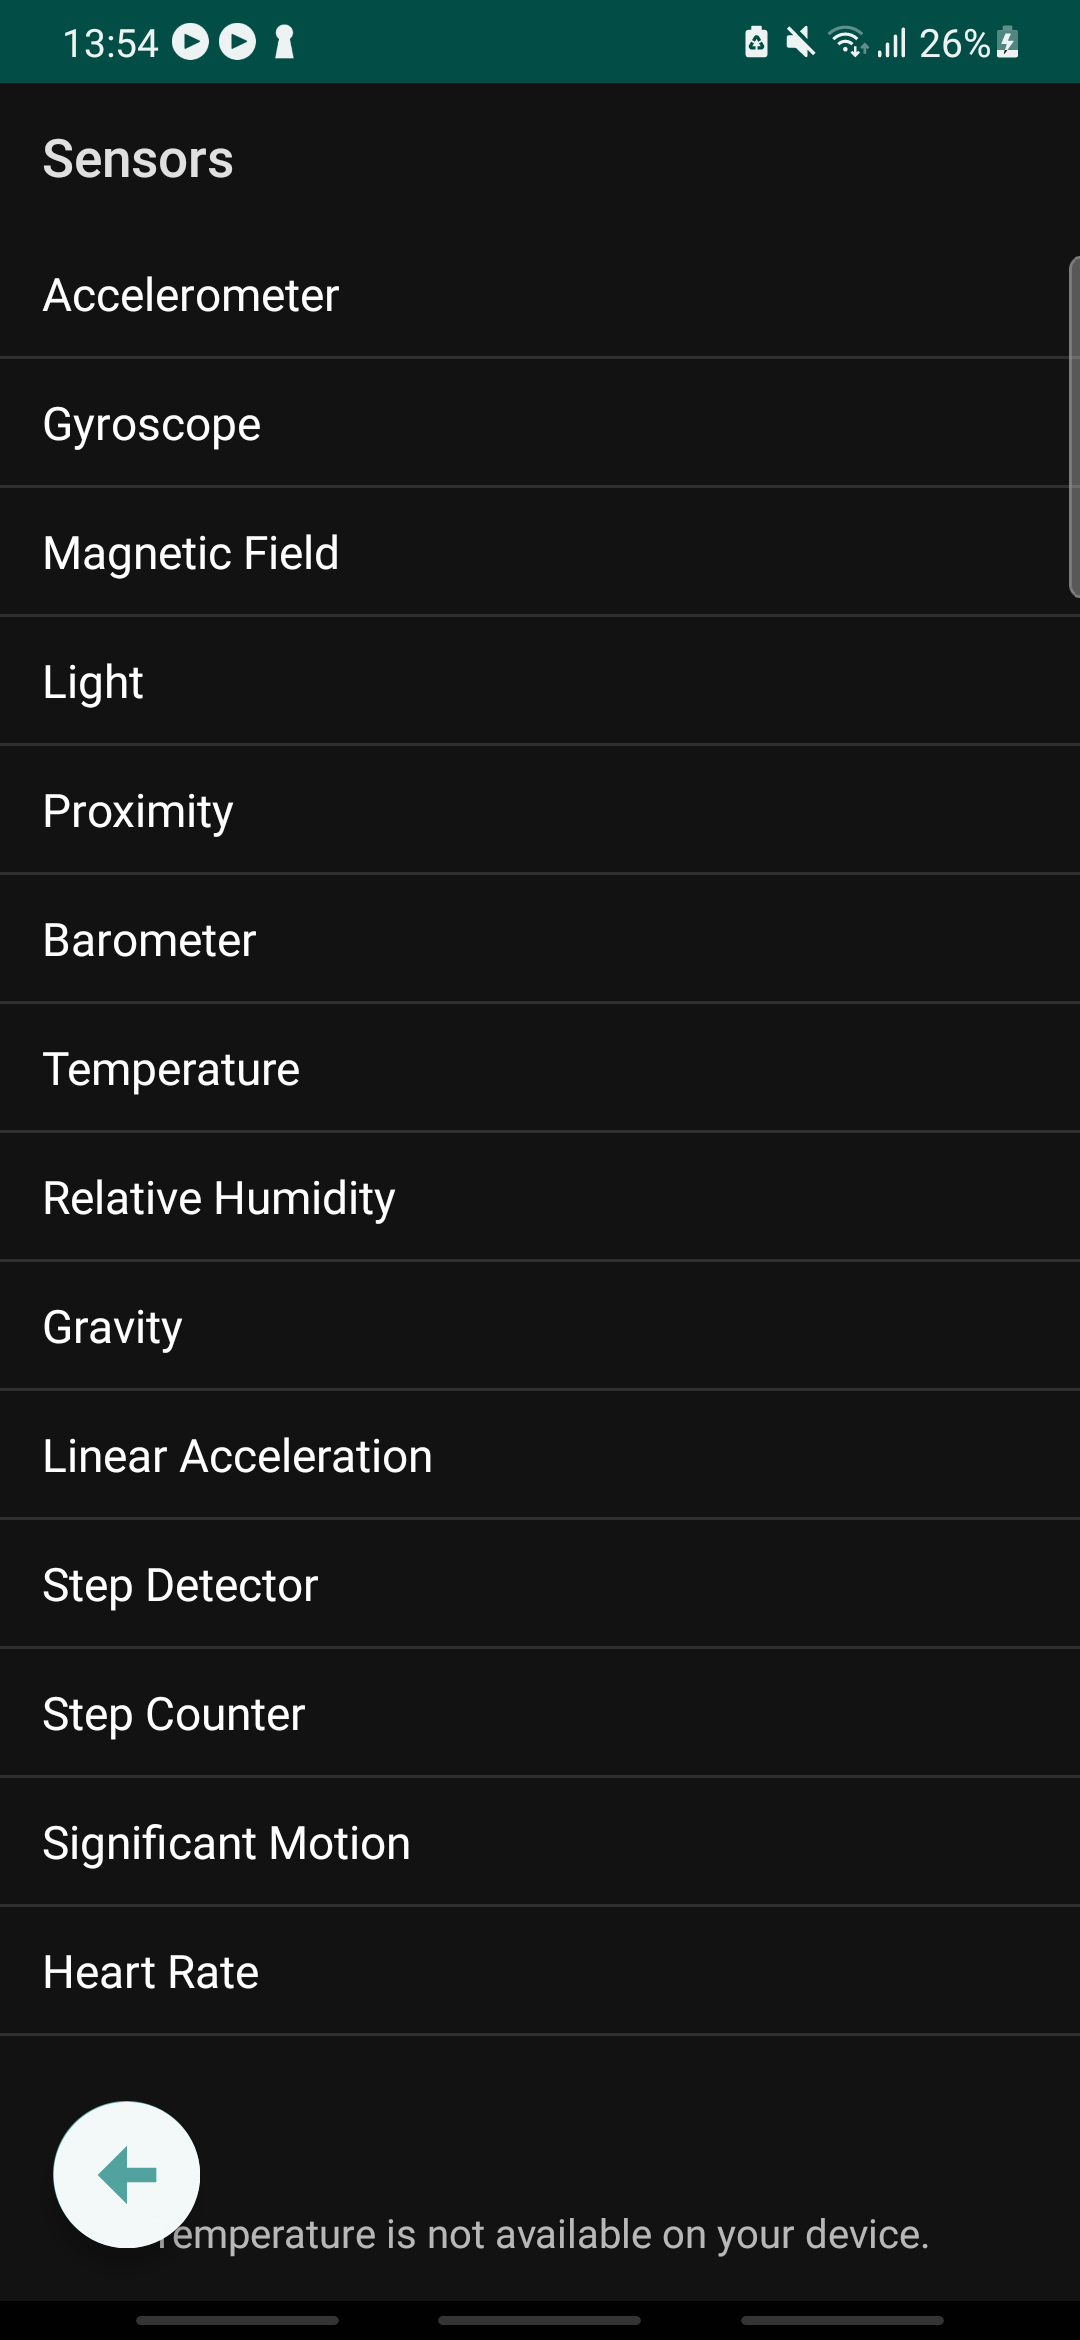
\includegraphics[height=.52\textwidth]{dispo/screenshotUnavailable}
            \paragraph{}
                Dans ce nouvel exercice, nous allons affiché la disponibilité \emph{(en bas de l'écran)} de un capteur en particulier.
            \paragraph{}
                Pour cela, nous réutilisons un ListView où chaque élément correspondra à un type de capteur. Puis nous redéfinissons la méthode \textbf{onItemClick()} pour modifier le comporter "cliquer" sur chaque item de la vue. La fonction nous donne en argument quelle item a été cliquer dessus sous forme d'un numéro d'index. On récupère le capteur qui correspond à cet index puis regarde si ce capteur est dispobile ou pas. C'est la fonction \textbf{getDefaultSensor()} qui nous inque qu'un capteur est indisponible quand il renvoie null.
                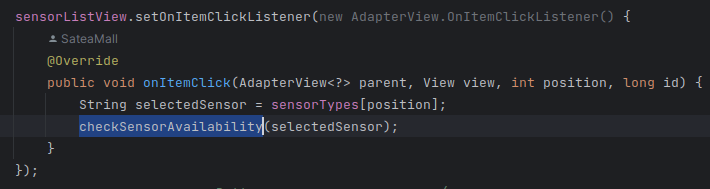
\includegraphics[width=.49\textwidth]{dispo/click}
                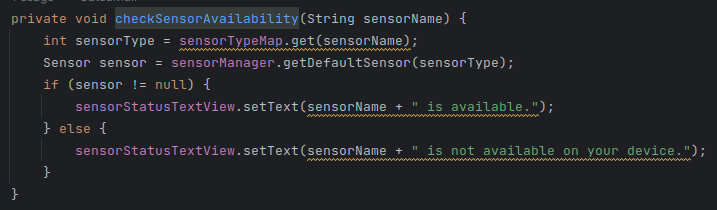
\includegraphics[width=.49\textwidth]{dispo/check}
        \section{Accéléromètre \emph{(Accelerometer)}}
            \paragraph{}
                Nous avons fait une petite application qui change la couleur en fond en fonction de l'accélération du téléphone.
            \paragraph{}
                Nous commençons par récupérer le sensorManager et le capteur accéléromètre. Afin de récupérer les données du capteur, il nous suffit de s'enregistrer (avec \textbf{registerListener()})auprès du service comme écouteurs d'événements et implémenter les méthodes de callback \textbf{onSensorChanged() et onAccuracyChanged()}.

                Nous choisissons d'utiliser \textbf{SensorManager.SENSOR\_DELAY\_UI} pour économiser de la batterie.

                Quand le capteur détecte un changement, la méthode \textbf{onSensorChanged()} est appelé. Si une accélération suffisament grande est détecté, on change la couleur du fond d'écran en rouge ou noir avec \textbf{view.setBackgroundColor()}.
                \includegraphics[width=.49\textwidth]{accelerometre/register}
                \includegraphics[width=.49\textwidth]{accelerometre/onSensorChanged}
        \section{Direction \emph{(Direction)}}
            \paragraph{}
                De façon très similaire à la section précédente, nous récupérons les capteurs qui nous intéresse et nous les écoutons.

                De même on implémente la méthode onSensorChanged afin d'implémenter le comportement que l'on souhaite. Lors d'un mouvment nous affichons dans quelle direction le smartphone se déplace. 
                
                Nous avons déclarer une balise TextView dans le layout correspondant à cette activité. On le récupère dans le code avec \textbf{directionTextView = findViewById(R.id.directionTextView);} puis on change le texte qu'il affiche avec du code : \textbf{directionTextView.setText("Left");}
                \includegraphics[width=.49\textwidth]{direction/screenshot}
        \section{Secouer un appareil \emph{(ShakeDevice)}}
            \paragraph{}
                Cette activité \emph{(ShakeDevice)} nous permet de faire basculer le flash entre allumé/éteint quand on second le smartphone.
            \paragraph{}
                Nous procédons comme dans les exercices précédent. On récupère le sensorManager. On récupère les capteurs (\emph{l'accéléromètre et la caméra}). On s'enregistre auprès de lui. Il faut remarquer qu'on doit d'abord récupérer le manger de caméra et utiliser un try catch car il est possible qu'on ait plusieurs ou 0 caméra.

                Nous avons choisit d'utiliser \textbf{SensorManager.SENSOR\_DELAY\_UI} pour pouvoir détecter les mouvments de manière plus fine.
                \includegraphics[width=.49\textwidth]{shake/register}
            \paragraph{}
                On implémente les méthodes de callback. On remarquera aussi l'utilisation de \textbf{System.currentTimeMillis()} pour empêcherque le flash ne s'allume et s'éteingne au cours du même mouvement.
                \includegraphics[width=.49\textwidth]{shake/onSensorChanged}
            \paragraph{}
                Si le smartphone est suffisament secoué, on fait basculer l'état du flash comme sur la capture d'écran suivante :
                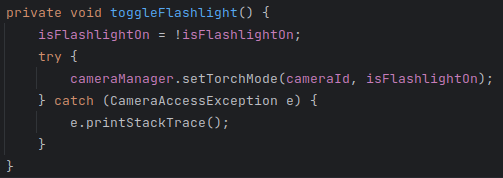
\includegraphics[width=.49\textwidth]{shake/toggle}
        \section{Proximité \emph{(Proximity)}}
            \paragraph{}
                Nous affichons une image indiquant si l'objet est proche ou loin.

                On récupère le sensorManager, le capteur et on s'enregistre auprès de lui encore une fois. On implémente les méthodes de callback. On déclare une \textbf{<ImageView>} dans le layout \emph{(activity\_proximity.xml)} qu'on mainupulera ensuite en java avec la mathode \textbf{setImageRessource()}.
                
                \noindent\includegraphics[width=.49\textwidth]{proximity/onSensorChanged}
                \noindent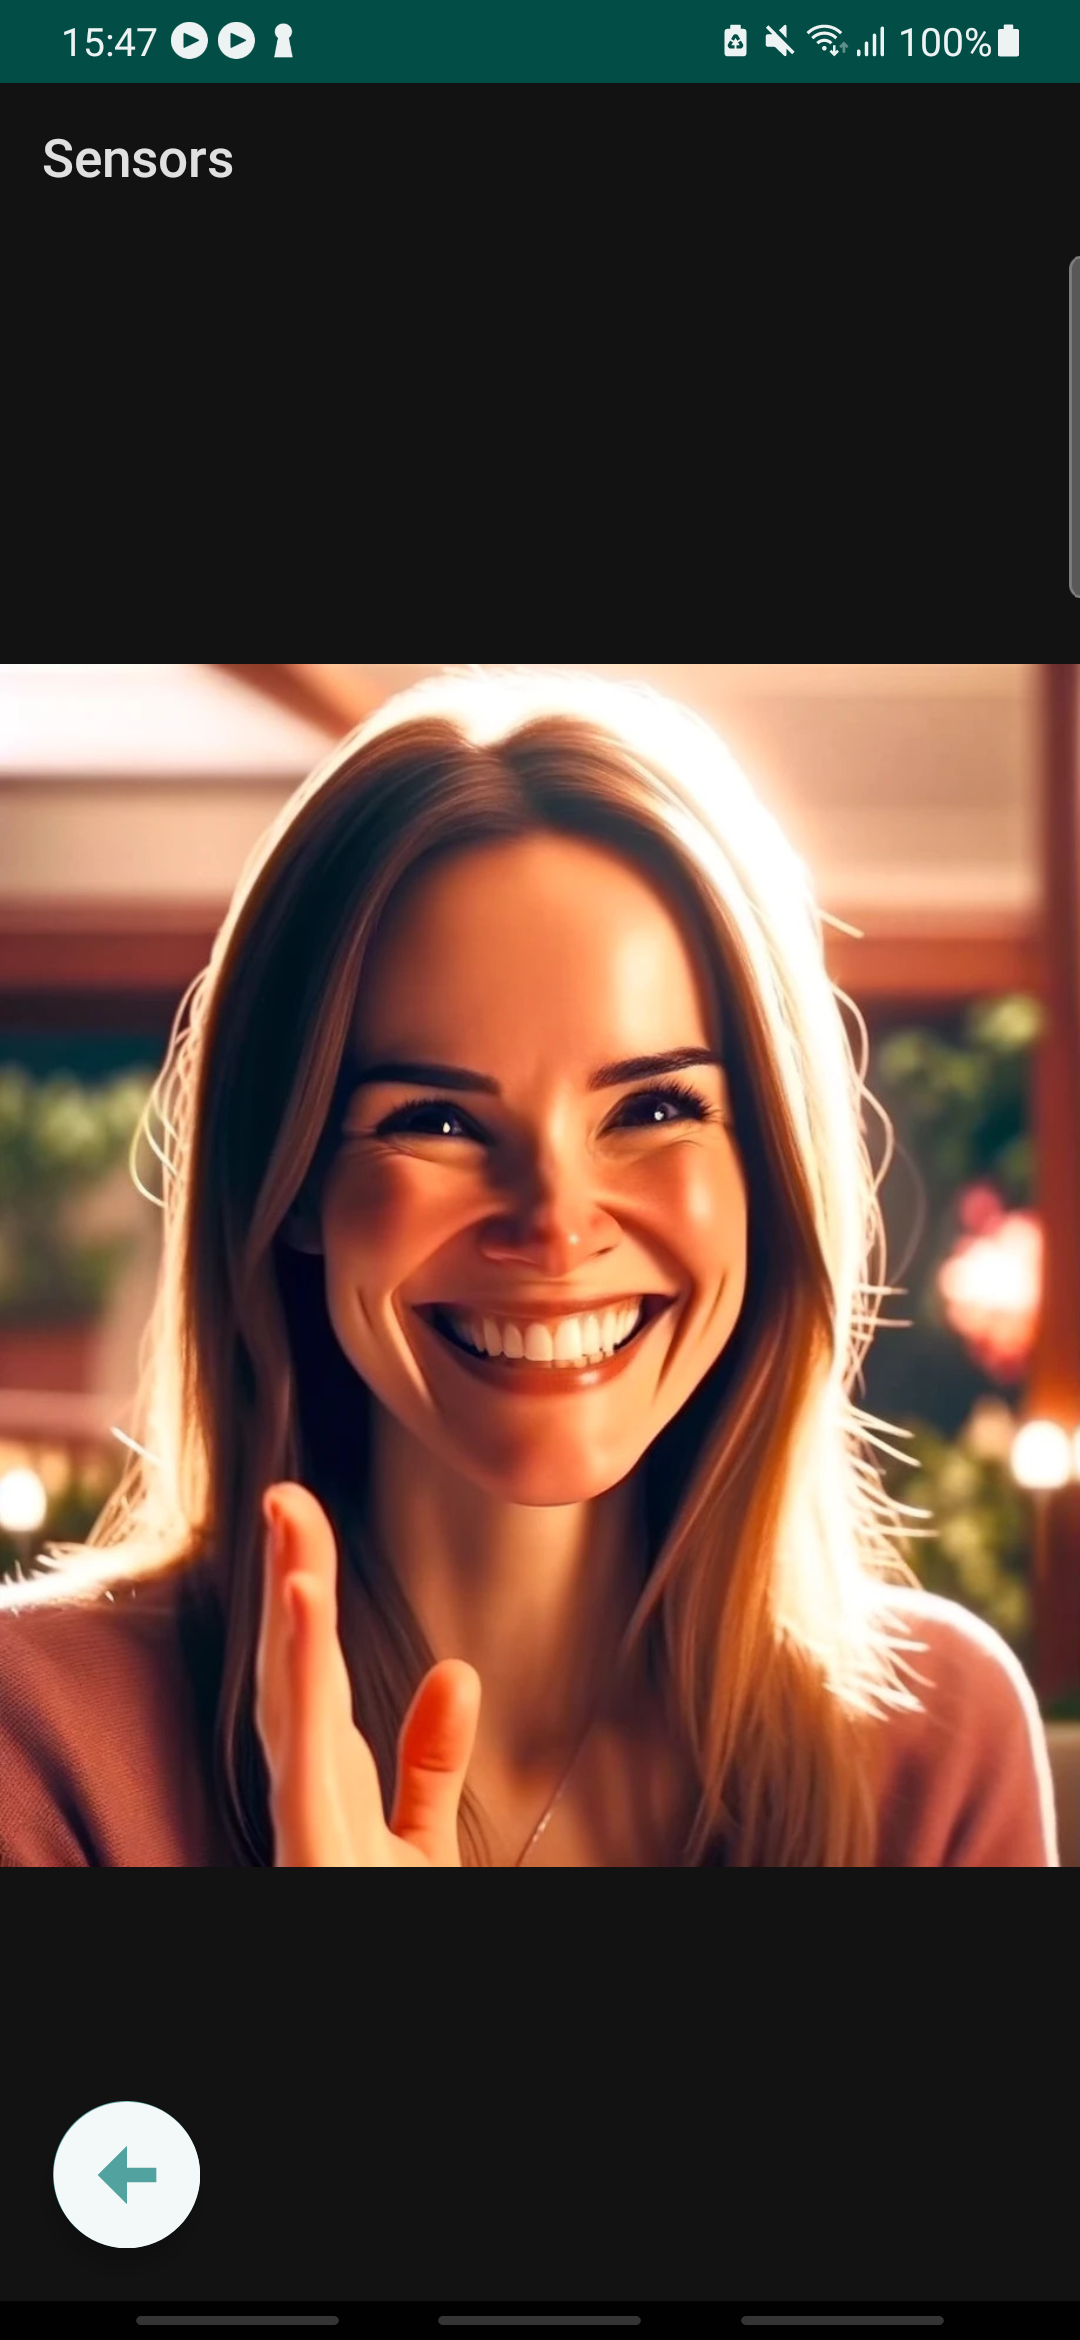
\includegraphics[height=.52\textwidth]{proximity/far}
                \noindent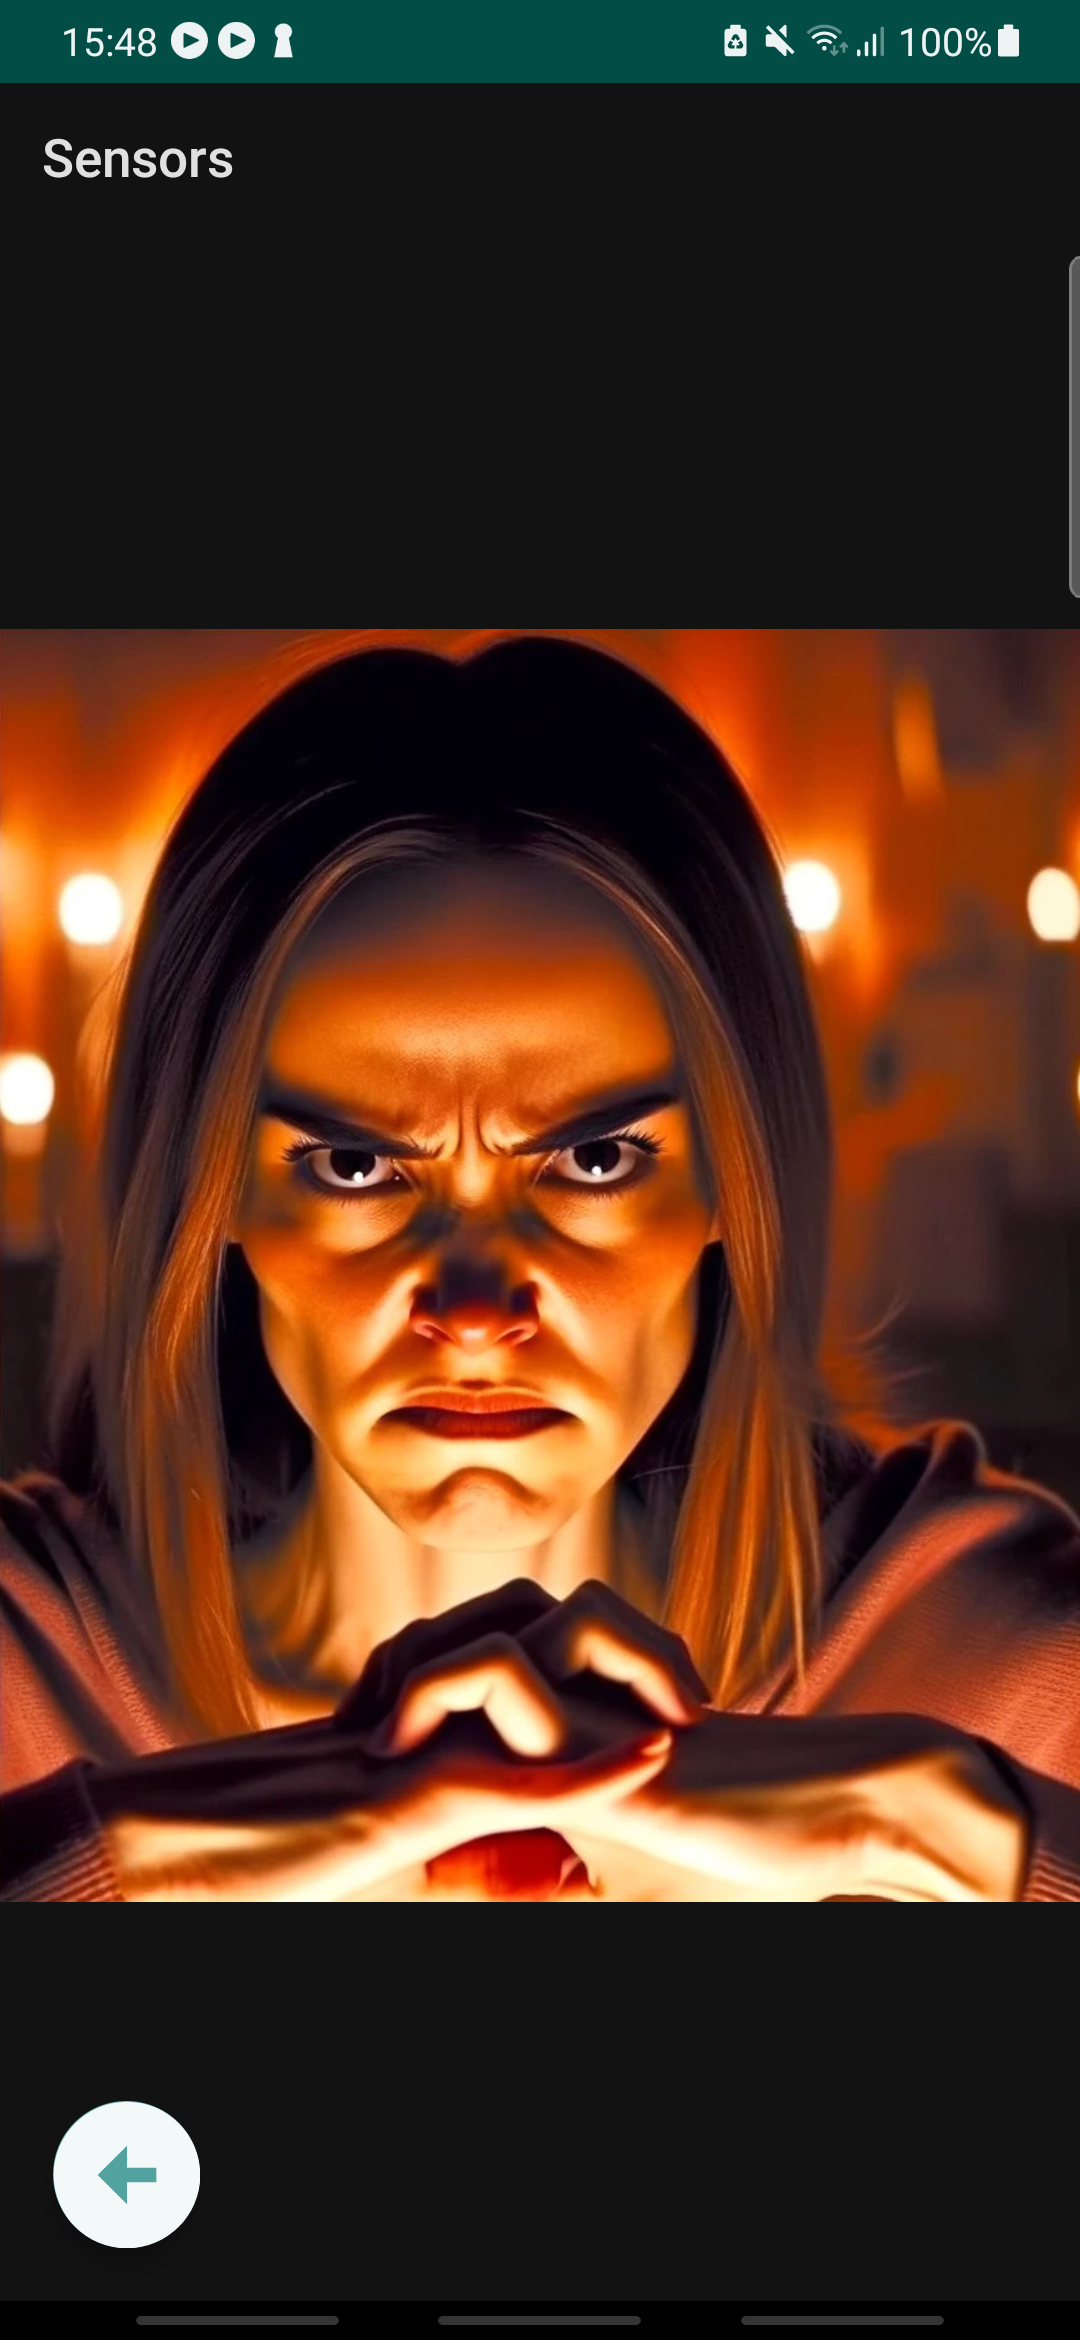
\includegraphics[height=.52\textwidth]{proximity/close}
        \section{Géolocalisation \emph{(Geolocation)}}
            \paragraph{}
                Dans de nombreuse application, il est souhaitable de connaitre la position de l'utilisateur. Pour ce faire, nous allons manipuler le gps.

            \paragraph{}
                Pour commencer nous accédons à un objet de type \emph{LocationManager} grâce à la fonction \textbf{getSystemService(Context.LOCATION\_SERVICE)}.
                \noindent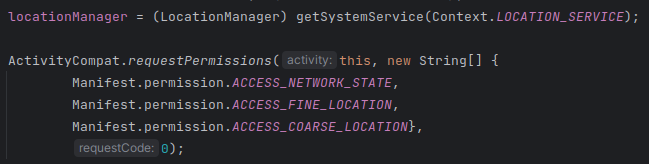
\includegraphics[width=.49\textwidth]{geo/request}

                Ensuite, on demande les permissions pour avoir la localisation de l'utilisateur.
                
                Puis, quand on reçoit l'autorisation (en redéfinissant \textbf{onRequestPermissionsResult}), On appel la fonction \textbf{getLastKnownLocation(GPS\_PROVIDER)} qui nous rend une \emph{Location}. Il nous suffit maintenant d'utiliser les fonctions \textbf{getLatitude() et getLongitude()}.
                \noindent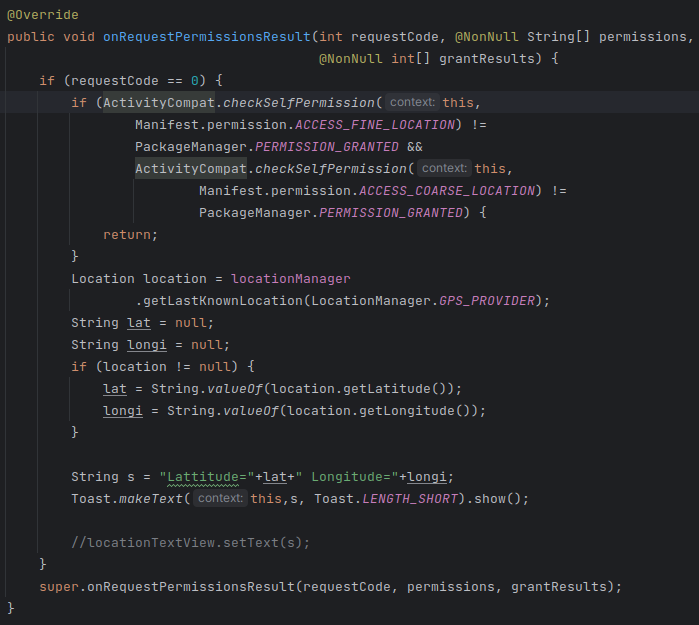
\includegraphics[width=.49\textwidth]{geo/onRequest}
                \noindent\includegraphics[width=.49\textwidth]{geo/screenshotSmall}
        \section{Extra}
            \subsection{Icone}
                \paragraph{}
                    Nous avons choisit de modifier l'îcone de notre application. Nous allons maintenant expliqué comment nous cela a été fait.

                \paragraph{}
                    Dans Android Studio, faire un click droit sur le dossier app. Aller dans New > Image Asset.
                    \noindent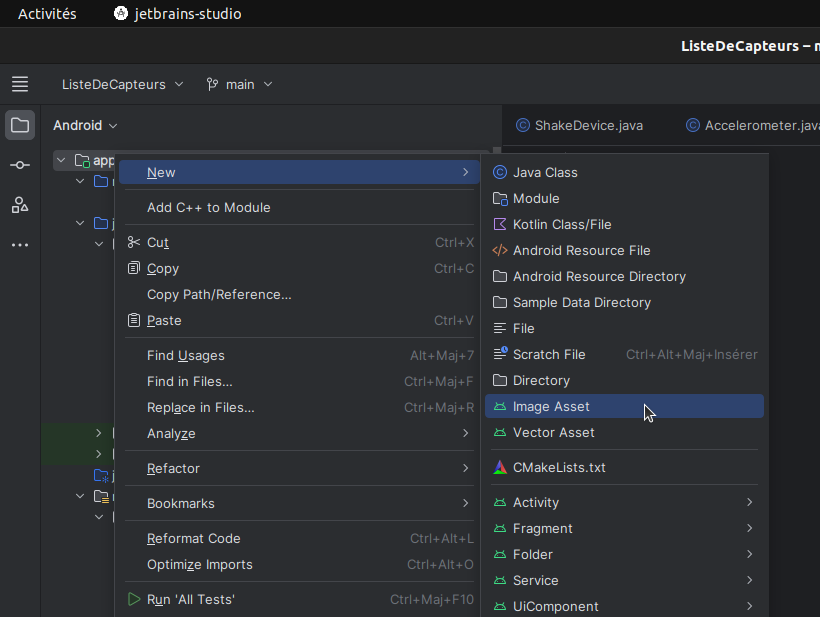
\includegraphics[width=.49\textwidth]{icone/imageAsset}
                    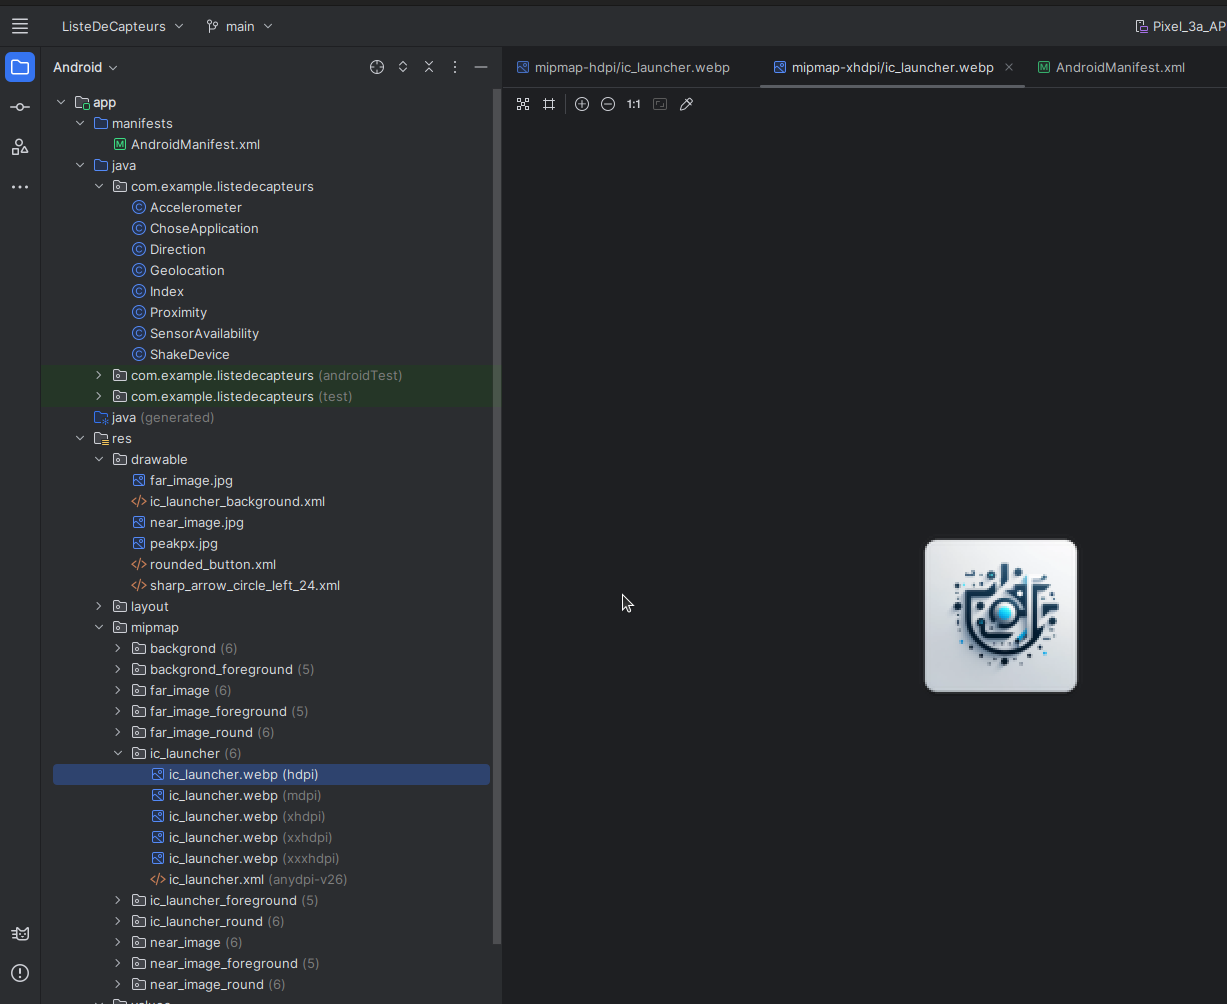
\includegraphics[width=.49\textwidth]{icone/res}
                    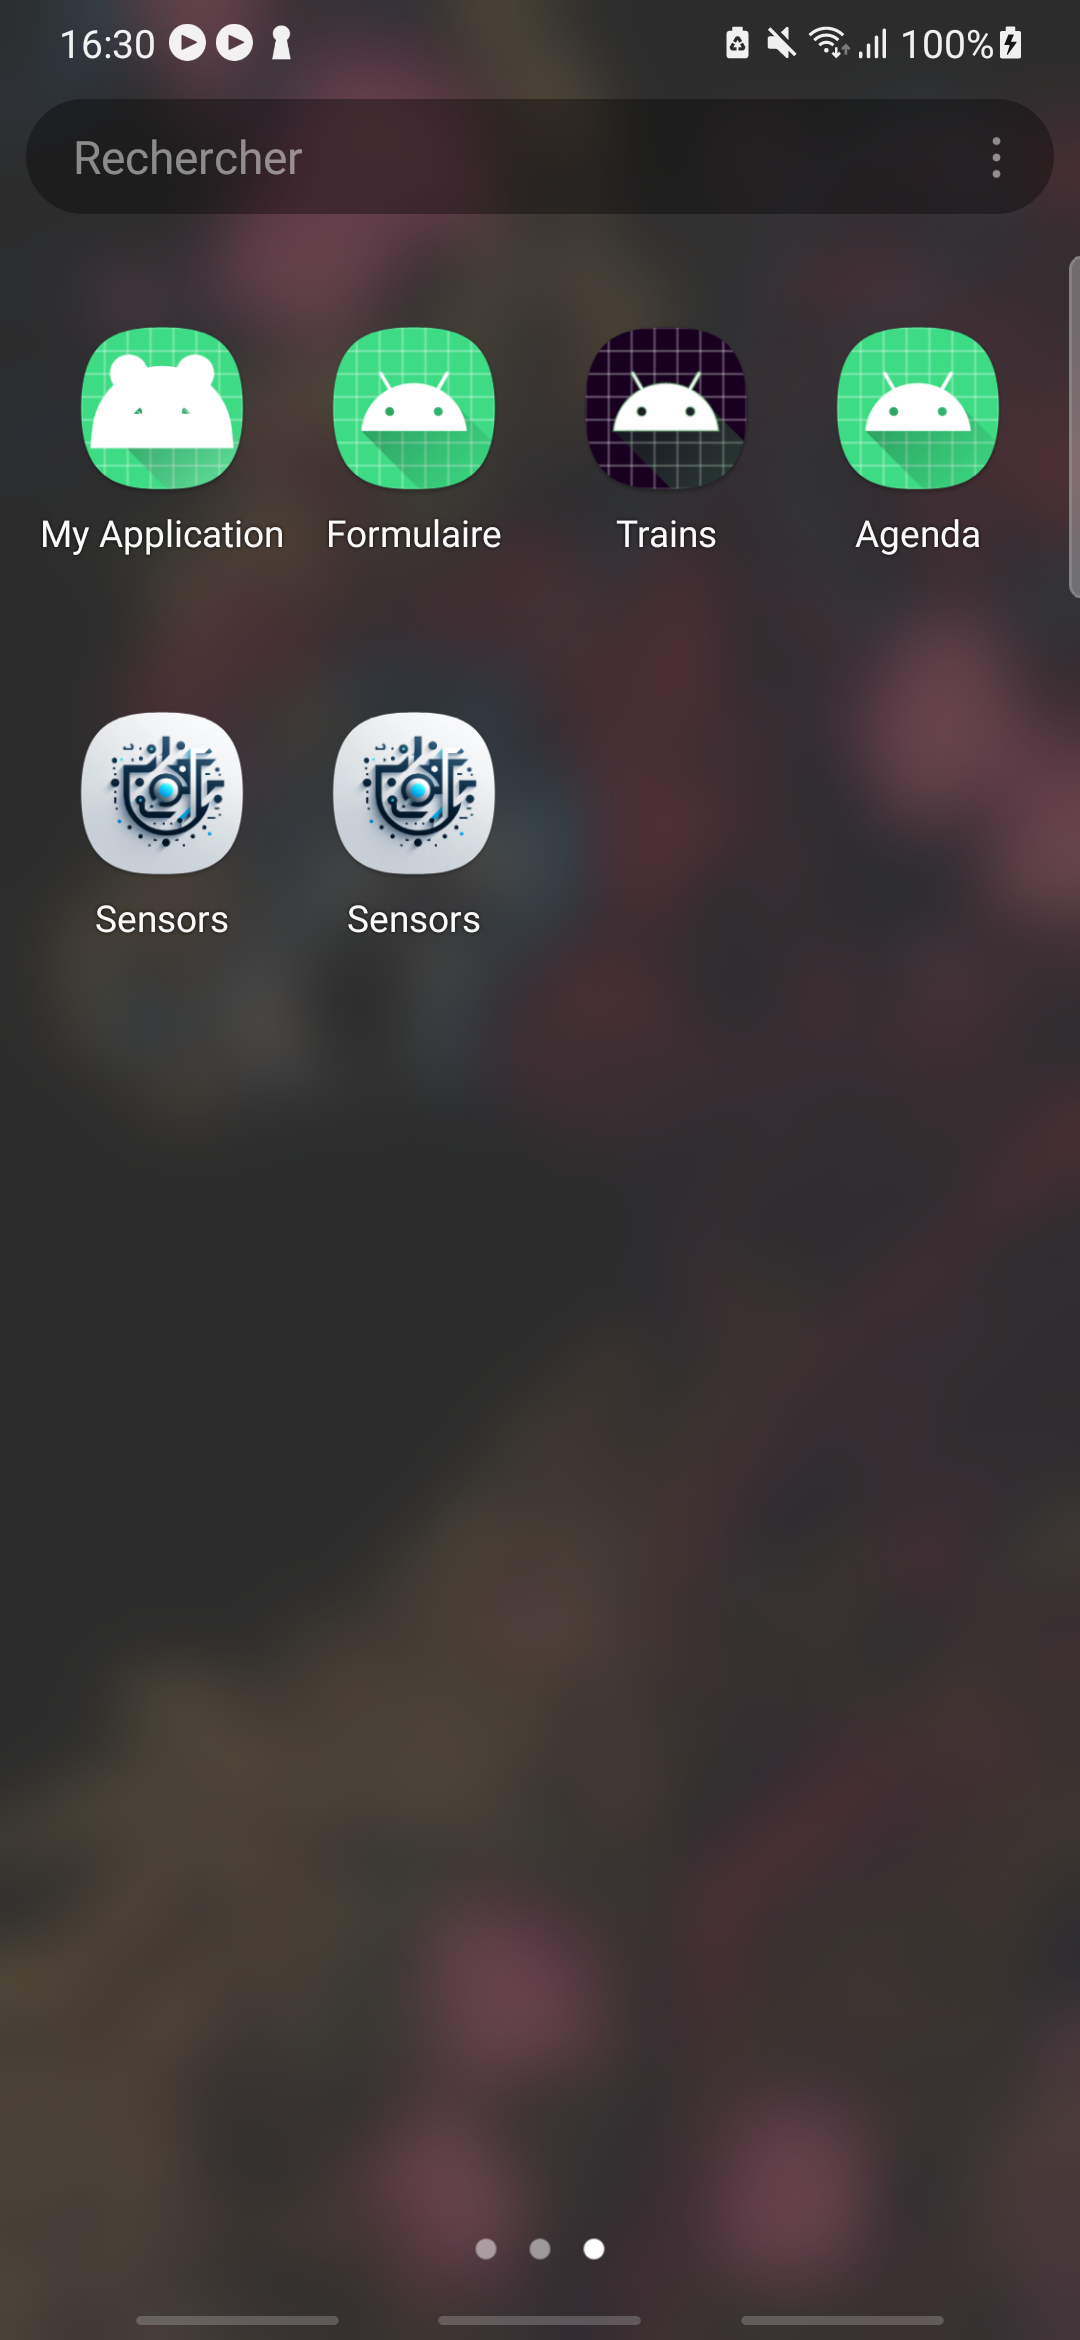
\includegraphics[height=.7\textwidth]{icone/drawer}
            \subsection{Retour}
                \paragraph{}
                    Nous avons placer un boutton de retour vers l'écran d'acceuil.
                    
                \paragraph{}
                    Dans le layout, nous ajoutons un boutton flottant (\emph{FloatingActionButton}) dans le coin inférieur gauche de la vue.
                    Et à l'aide des connaissances du 1er tp, on redéfinit la méthode \textbf{onClick()}. On comment l'activité correspondant à l'acceuil avec un \textbf{Intent} et la méthode textbf{startActivity()}.

                    \noindent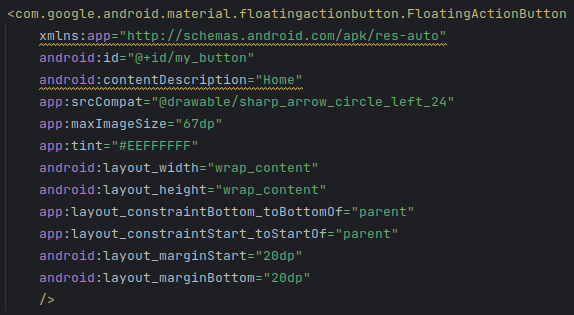
\includegraphics[width=.49\textwidth]{button/boutton}
                    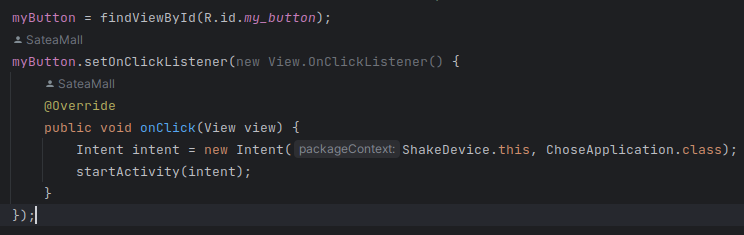
\includegraphics[width=.49\textwidth]{button/onClick}

    \end{multicols}
\end{document}